

%\usepackage{graphicx}
\usepackage{hyperref}
\usepackage{todonotes}

\usepackage{endfloat}
\renewcommand{\efloatseparator}{\mbox{}} % no new page between figures

\usepackage{booktabs} % For formal tables

\settopmatter{printacmref=false} % Removes citation information below abstract
\renewcommand\footnotetextcopyrightpermission[1]{} % removes footnote with conference information in first column
\pagestyle{plain} % removes running headers

\newcommand{\TODO}[1]{\todo[inline]{#1}}



\title{Visualization in Big Data}


\author{Himani Bhatt}
\affiliation{%
  \institution{Indiana University}
  \city{Bloomington} 
  \state{Indiana} 
}
\email{himbhatt@iu.edu}



% The default list of authors is too long for headers}
\renewcommand{\shortauthors}{H. Bhatt}



\begin{abstract}
Data Visualization is the term used for knowing the visual context of data in order to understand its significance. How to unravel the strands of big data to pick out the relevant parts. If we have multiple sources of data how do we know where to look. Data visualization is the solution to all these questions. It helps to convert information into knowledge. Businesses are using big data in order to better understand their customers and to optimize their business processes. In order to find the meaning, tell the story and sharing the story, visualization is needed where data meets design.
\end{abstract}

\keywords{ HID $202$, i$523$, BI(Business Intelligence), DV(Data Visualization).}

\maketitle

\section{Introduction} 

Data visualization is emerging as an important fusion of graphics, scientific visualization, database and human-computer interaction. Data visualization if properly aligned can provide a shorter route for decision making and a way of conveying critical information. For the data visualization to be truly productive, it has to be interactive, meaningfull, understandable, user friendly and approachable. The main advantage of data visualization is that it provide insights into complex data sets by communicating their key aspects \cite{Intro01}.Not only insights, it allows users to see different perspective of the data, offers ability to note exceptions in the data, equips users with ability to see influences that would be difficult to find otherwise, helps users finding nuances that are significant \cite{Intro02}. \\

According to Friedman (2008) the ``main goal of data visualization is to communicate information clearly and effectively through graphical means. It doesn't mean that data visualization needs to look boring to be functional or extremely sophisticated to look beautiful. To convey ideas effectively, both aesthetic form and functionality need to go hand in hand, providing insights into a rather sparse and complex data set by communicating its key-aspects in a more intuitive way. Yet designers often fail to achieve a balance between form and function, creating gorgeous data visualizations which fail to serve their main purpose $-$ to communicate information'' \cite{Intro03}.\\

Simple form of data visualization include graphs, pi charts, histograms, scatter plots, and maps. Colors can be used to show correlation, size to show quantity, and orientations used to show trends. Design is used to better communicate varied sorts of information, processes, hierarchy, anamoly and analogy. Tables \ref{table1} and \ref{table2} shows basic type of visualization diagrams with their usage.



\begin{table}[H]

\centering
\begin{adjustbox}{max width=\textwidth}

  \begin{tabular}{ | c | m{3cm} | m{3cm} | }
    \hline
    Data visualization diagrams & Interpretation \\ \hline
    \begin{minipage}{.3\textwidth}
      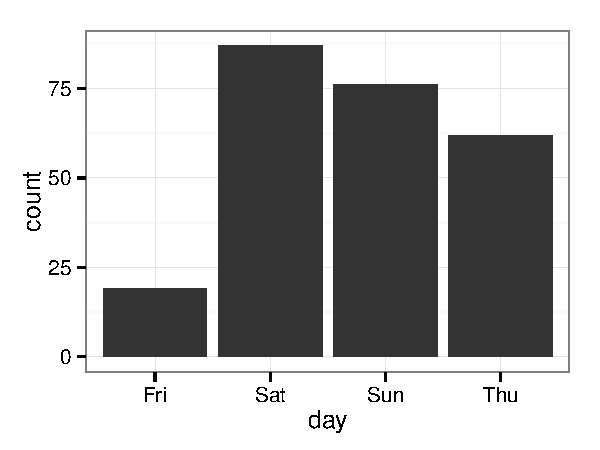
\includegraphics[width=30mm, height=30mm]{images/barchart.pdf}
      \caption*{figure}{Barchart}
    \end{minipage}
    &
    %\begin{minipage}[t]{3cm}
      Used for comparison of variables against single variable.
          %\end{minipage}
    
    \\ \hline
    
    \hline
  
    \begin{minipage}{.3\textwidth}
      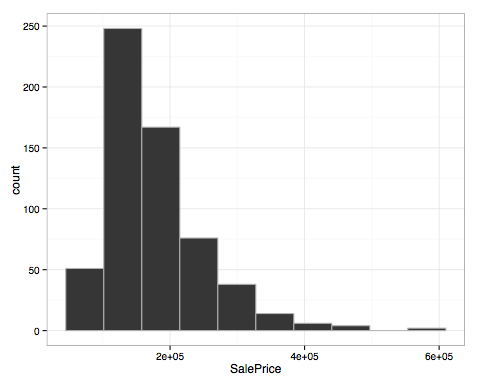
\includegraphics[width=30mm, height=30mm]{images/histogram.png}
      \caption*{figure}{Histogram}
    \end{minipage}
    &
    %\begin{minipage}[t]{3cm}
      Histogram shows frequency of score occurrences in a continuous data set that has been divided into classes, called bins.
    %\end{minipage}
    
    \\ \hline
    
   \hline
  
    \begin{minipage}{.3\textwidth}
      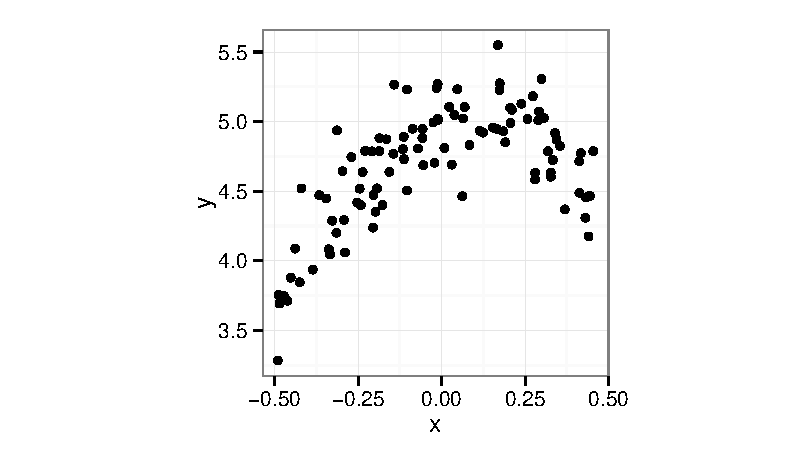
\includegraphics[width=30mm, height=30mm]{images/Scatterplot.pdf}
      \caption*{figure}{Scatter Plot}
    \end{minipage}
    &
    %\begin{minipage}[t]{3cm}
      Scatter plot is used to show correlation between two variables.
          %\end{minipage}
    
    \\ \hline
    
    \hline
  
    \begin{minipage}{.3\textwidth}
      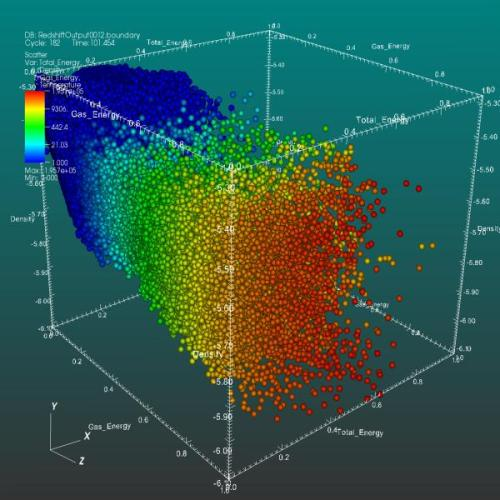
\includegraphics[width=30mm, height=30mm]{images/Scatter_plot3D.jpg}
      \caption*{figure}{3D Scatter Plot}
    \end{minipage}
    &
    %\begin{minipage}[t]{3cm}
      3D Scatter plot is used to show correlation between three variables.
          %\end{minipage}
    
    \\ \hline
    
    \hline
  
    \begin{minipage}{.3\textwidth}
      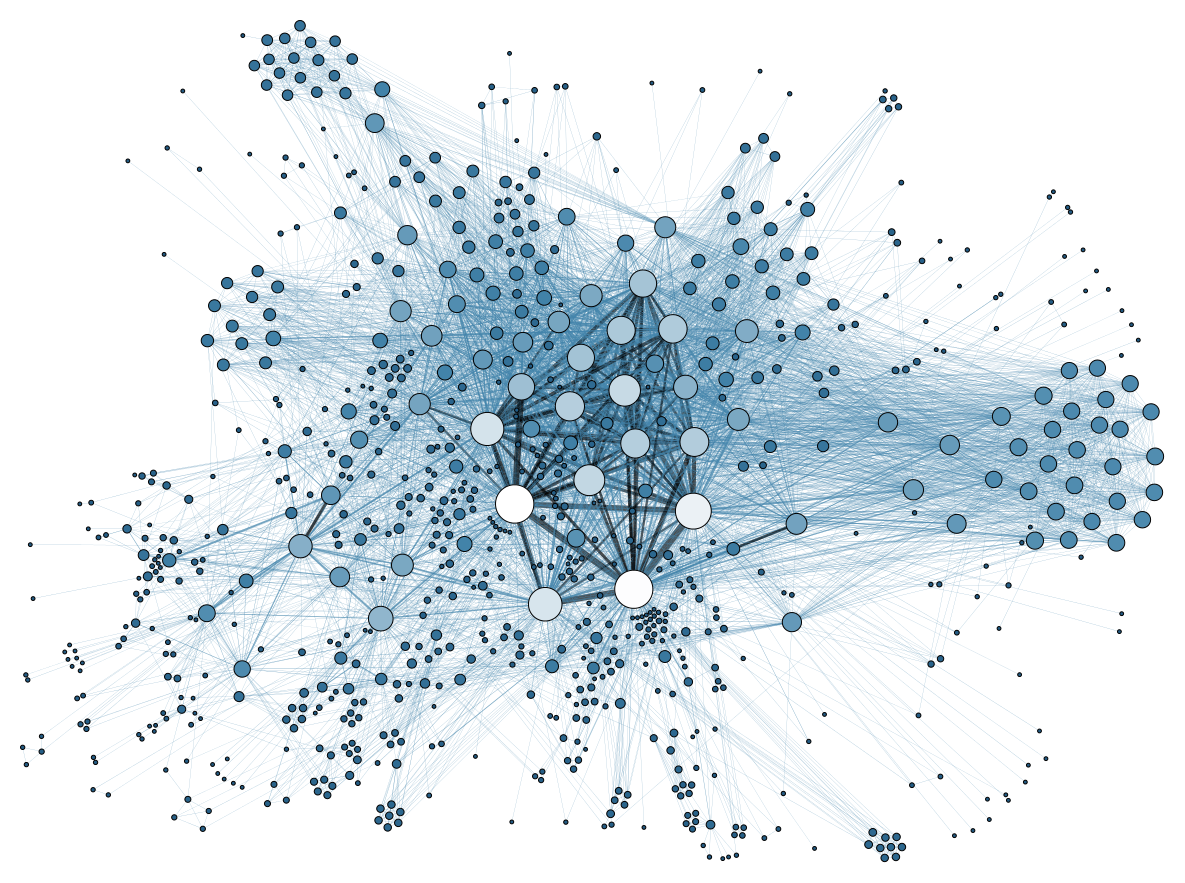
\includegraphics[width=30mm, height=30mm]{images/Network.png}
      \caption*{figure}{Network}
    \end{minipage}
    &
    %\begin{minipage}[t]{3cm}
      Networks are used for finding clusters in the network, discovering bridges in the network, in determining most influential nodes and in finding outliers who are out of periphery of network.
          %\end{minipage}
    
    \\ \hline
    
  \end{tabular}
  \end{adjustbox}

  \caption{Data visualization diagrams. \cite{Table01}}\label{table1}
\end{table}





\begin{table}[H]
\label{table2}
  \centering
  \begin{adjustbox}{max width=\textwidth}
  \begin{tabular}{ | c | m{3cm} | m{3cm} | }
    \hline
    Data visualization diagrams & Interpretation \\ \hline
    \begin{minipage}{.3\textwidth}
      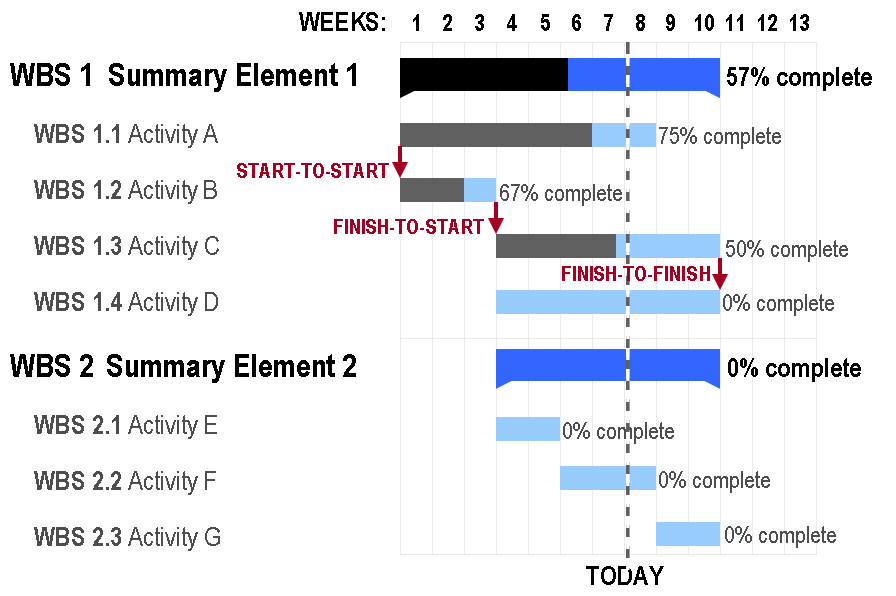
\includegraphics[width=30mm, height=30mm]{images/GanttChart.png}
      \caption*{figure}{Gantt chart}
    \end{minipage}
    &
    %\begin{minipage}[t]{3cm}
      A Gantt Chart is used as a project management tool to illustrate how the project will run. We can view individual tasks, their duration and the sequencing of these tasks.
          %\end{minipage}
    
    \\ \hline
    
    \hline
  
    \begin{minipage}{.3\textwidth}
      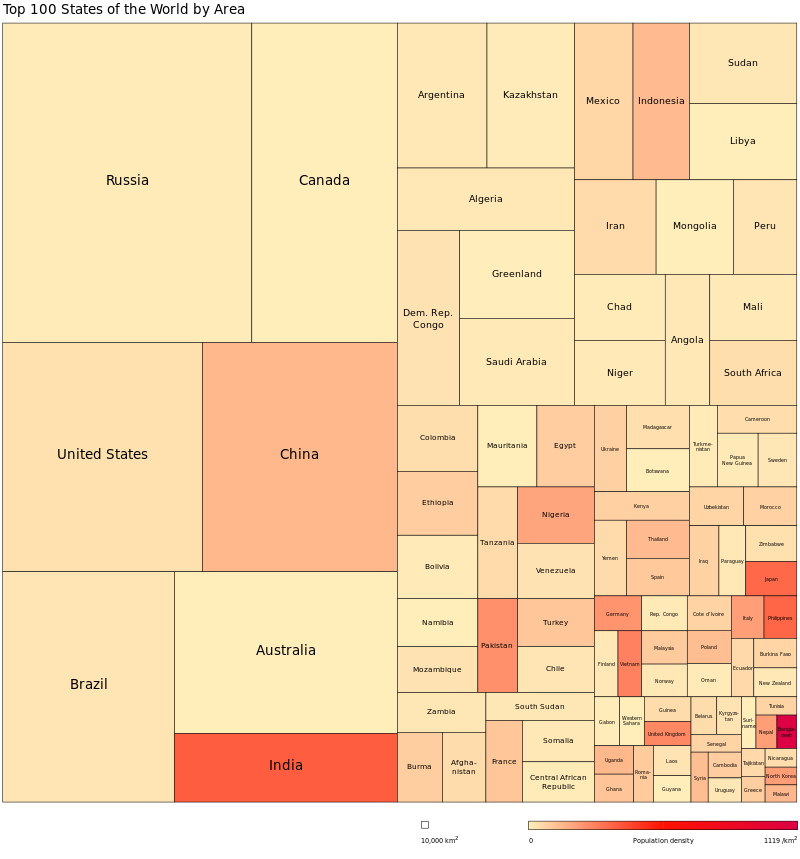
\includegraphics[width=30mm, height=30mm]{images/Treemap.png}
      \caption*{figure}{Treemap}
    \end{minipage}
    &
    %\begin{minipage}[t]{3cm}
      Treemaps are ideal for displaying large amounts of hierarchically structured (tree-structured) data.
    %\end{minipage}
    
    \\ \hline
    
   \hline
  
    \begin{minipage}{.3\textwidth}
      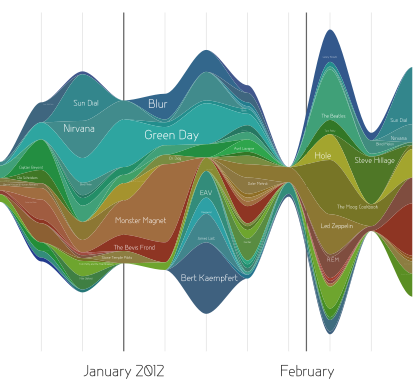
\includegraphics[width=30mm, height=30mm]{images/Streamgraph.png}
      \caption*{figure}{Stream graph}
    \end{minipage}
    &
    %\begin{minipage}[t]{3cm}
      Stream graph are used to show changes of different categories over time when there are many categories and these categories start and stop at different times. 
    %\end{minipage}
    
    \\ \hline
    
    \hline
  
    \begin{minipage}{.3\textwidth}
      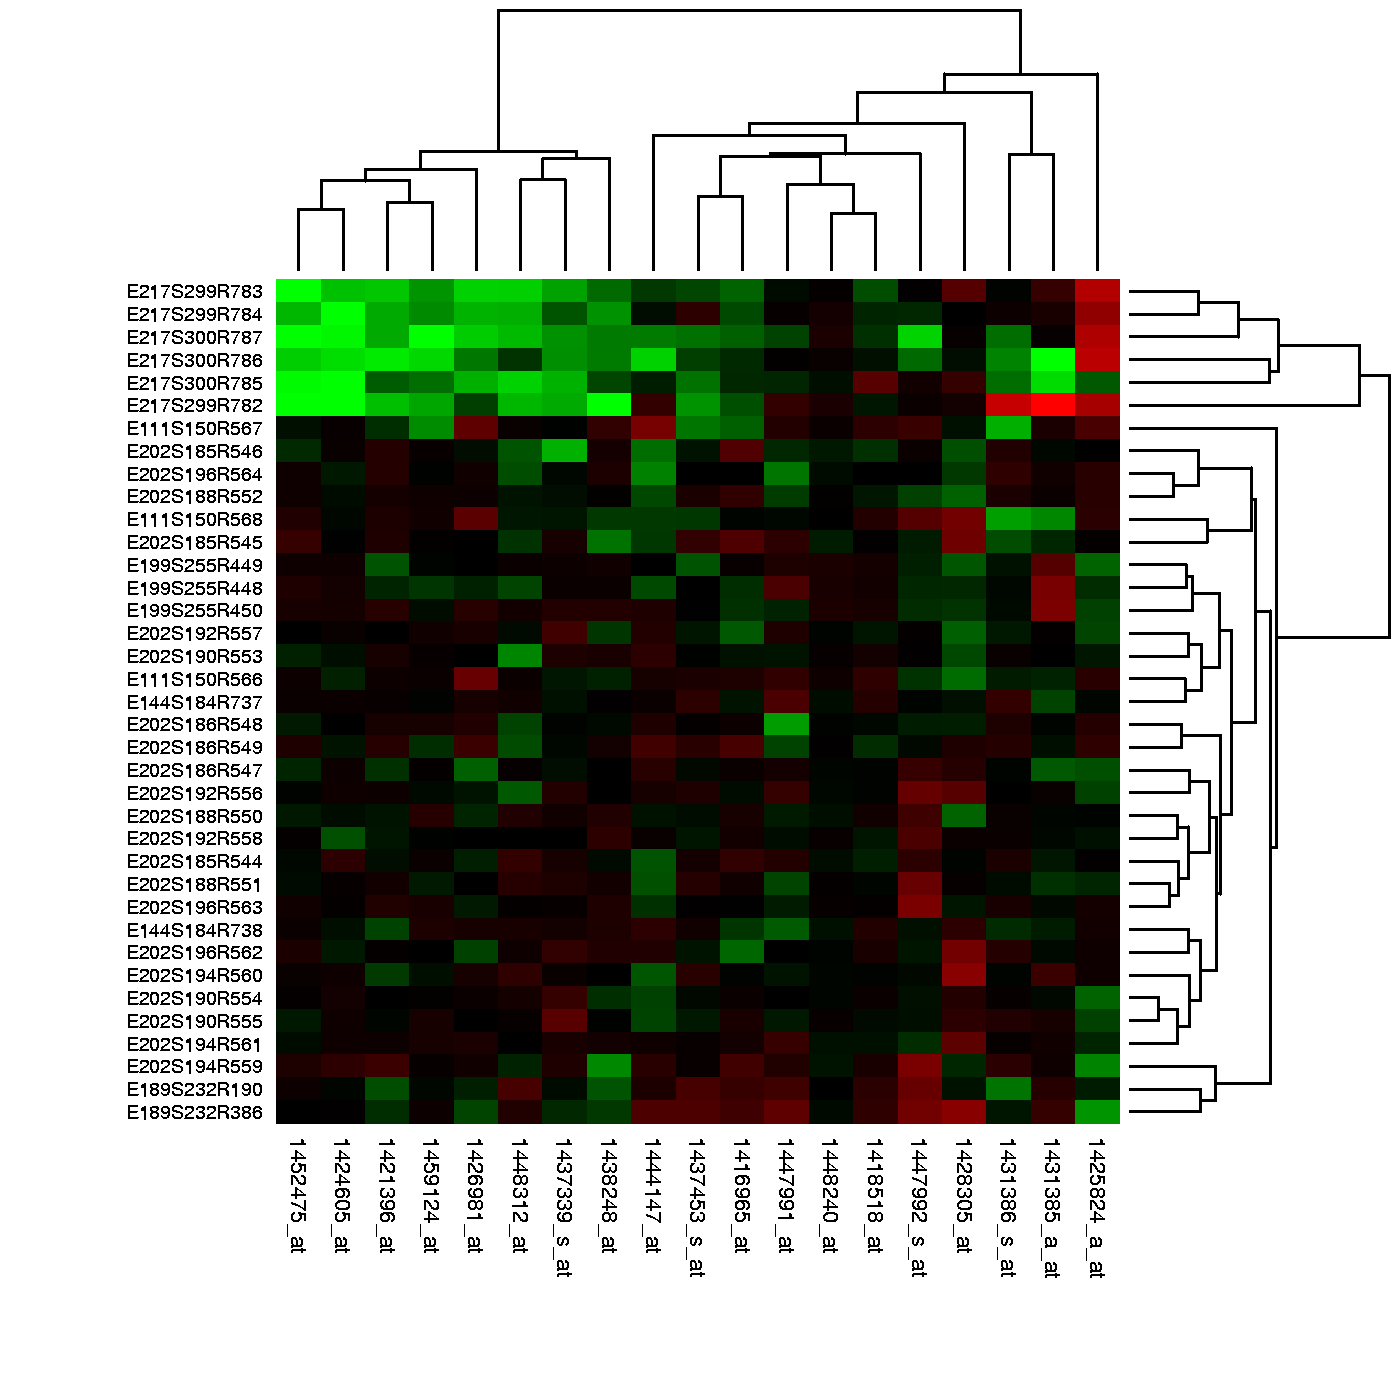
\includegraphics[width=30mm, height=30mm]{images/Heatmap.png}
      \caption*{figure}{Heatmap}
    \end{minipage}
    &
    %\begin{minipage}[t]{3cm}
      A heat map is a two-dimensional representation of data in which values are represented by colors.
          %\end{minipage}
    
    \\ \hline
    
  
  \end{tabular}
   \end{adjustbox}
  \caption{Data visualization diagrams \cite{Table01}} \label{table2}
\end{table}


\section{Data Visualization Tools}

Visualization solutions are rapidly evolving. Some of the most popular and innovative data visualization tools are : \\
\subsection*{Tableau}

Tableau is a data visualization tool created by Tableau Software. Tableau’s data visualization is considered to be more interactive than the ones provided by the general BI solutions. The huge and fast changing datasets used in big data operations, artificial intelligence and machine learning can be handled efficiently because of the integration of tableau with various advance database solutions like Teradata, SAP, Amazon AWS, Hadoop. Tableau offers 5 main products: Tableau Desktop,Tableau Server, Tableau Online, Tableau Reader, Tableau Public \cite{Tableau}.\\

\subsection*{Qlikview}

Qlikview is the business discovery platform. It offers powerful business intelligence, analytics and enterprise reporting capabilities other than the data visualization capabilities. It has a clean and clutter free user interface. It is used with Qliksense, which is responsible for data exploration and discovery. Dynamic calculation is the major innovation in Qlikview. It generate new views of information as the users clicks or taps, and instantly responds with the newly calculated set of data and visualizations \cite{Qlikview}.\\

\subsection*{Spotfire}

Tibco spotfire is the tool used for business intelligence. It is used by predictive analytics professionals to make imperative decisions. It has a library that helps in transferring analysis that has occurred by hard practices from an expert to business user. It not only increase the speed of decision making but also delivers framework for circulation of analysis applications, that depends on the needs of an association. It also make access to the server based data sources easy, since it has its own analytics servers centrally coped information facilities. It has self configuring visual data analysis environment that helps users to explore, visualize and query data in real time \cite{Spotfire}.\\

\subsection*{MS BI Stack}

Microsoft BI Stack provides all the tools we need to build, manage and use a BI solution, as part of Microsoft SQL Server, Sharepoint and Office applications. Visual studio 2015 can be used to get business insights on a platform that is designed to work with the data, systems and tools. For the enterprises using Microsoft technologies, Microsoft BI stack seems to be the most logical extension. Microsoft has products for data integration(SSIS), analytics(SSAS), business intelligence(SSRS), and visualization. These tools can be used as a stand alone tool or it can be integrated with sharepoint system or MS office desktop products(like Excel) \cite{MS}.


\section{Comparison of Data Visualization products}

Big data can be best comprehended using interactive Data Visualization which has drill down capabilities and dashboards. Among the several DV products available in the market, each has its place. For example, Spotfire has best web client and analytical functionality, Qlikview has best interactive drilldown capabilities, Microsoft BI platform gives best price performance ratio, whereas Tableau has best ability to interact with OLAP cubes \cite{compare}.\\ The table will show these 4 DV product comparison on the basis of business and technical criteria :







\begin{acks}

  The author would like to thank Dr. Gregor von Laszewski and the Assistant Instructors for their feedback and help.
\end{acks}

\bibliographystyle{ACM-Reference-Format}
\bibliography{report} 



